%!TEX root = ../SciVis.tex

The aim of this step is for you to understand and implement the height plot technique. Height plots are typically used to visualize scalar functions defined over (planar) 2D domains by plotting the function values along the third (z) dimension. In this step, you have to implement the height plot technique, and use this mechanism to visualize the various scalar fields which have already been computed during the previous steps. Specifically, you have to visualize the fluid density rho, the velocity magnitude | v |, and the force magnitude | f |. Proceed as follows:
 
 
 
·        Implement the height plot algorithm atop of the simulation grid. That is, use the already existing simulation grid geometry as base plane for the height plot. The plot will be hence drawn in 3D, atop (or below) of this plane. The ‘input’ of the plot should be user settable, i.e. one of the scalar fields named above. Of course, the plot should dynamically change with the simulation.


\begin{figure}[htbp]
\centering
\begin{minipage}[t]{0.48\textwidth}
        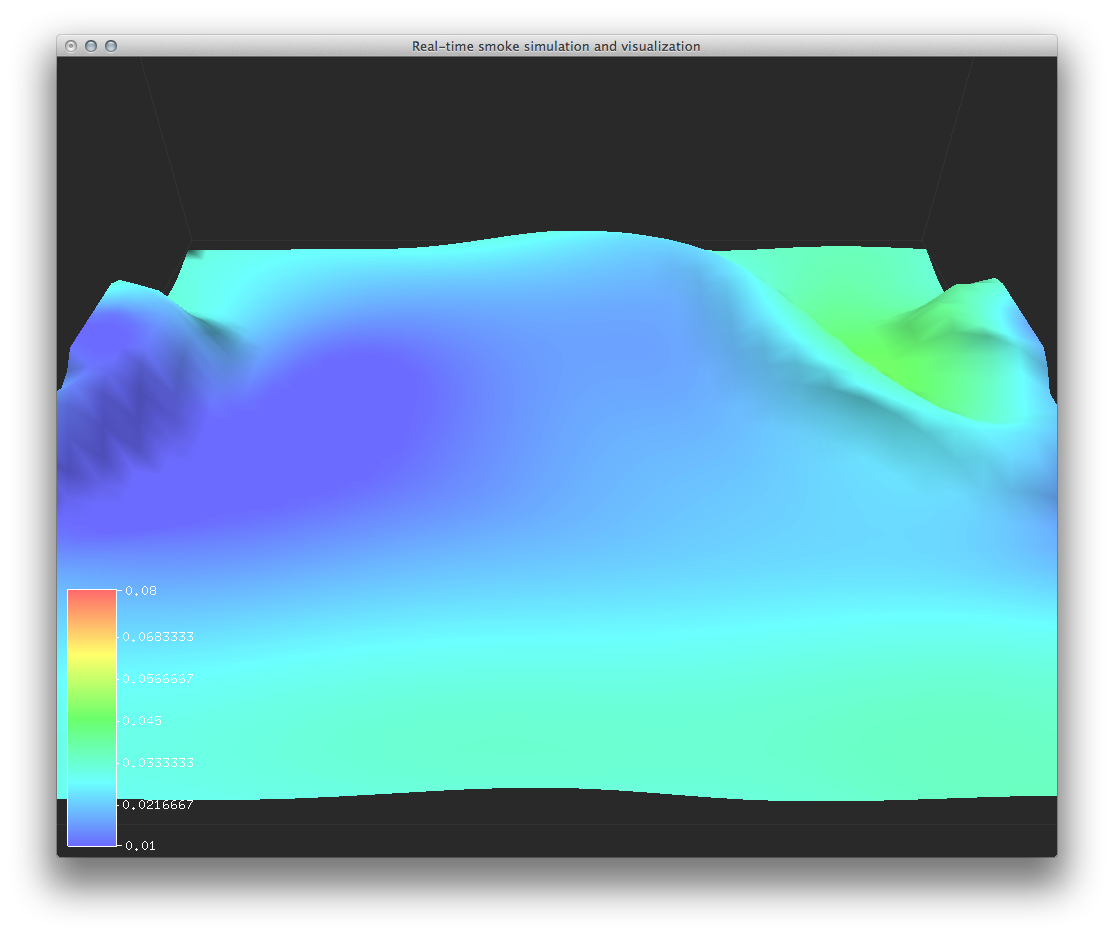
\includegraphics[height=3in]{figures/colormaps/densityvelocity.png}
\caption{Fluid density visualized with a heat colormap}
\label{fig:heatmap}
\end{minipage}\hspace{.04\textwidth}%
\begin{minipage}[t]{0.48\textwidth}
        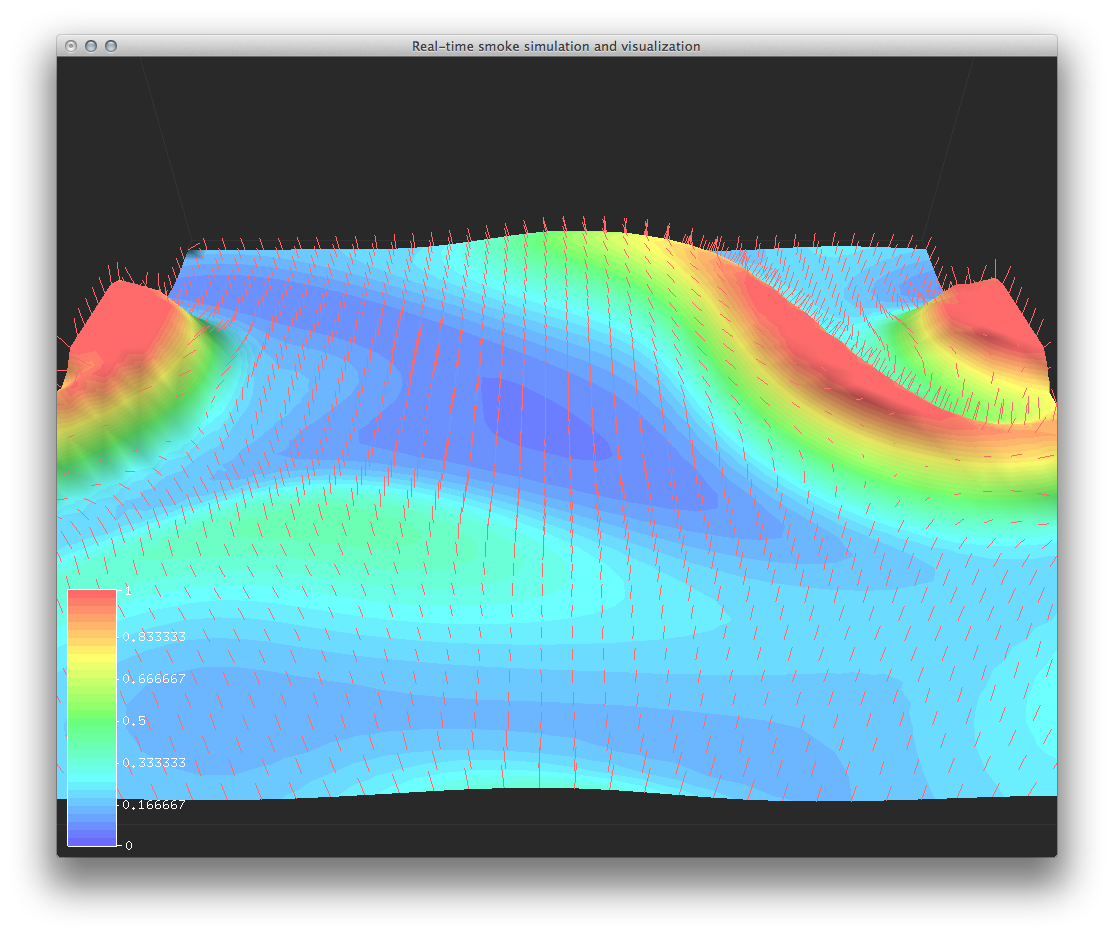
\includegraphics[height=3in]{figures/colormaps/densitynormals.png}
    \caption{Heat colormap with a reduced number of colors. The color banding effect is clearly visible.}
    \label{fig:banding}
\end{minipage}
\end{figure}

\begin{figure}[htbp]
    \centering 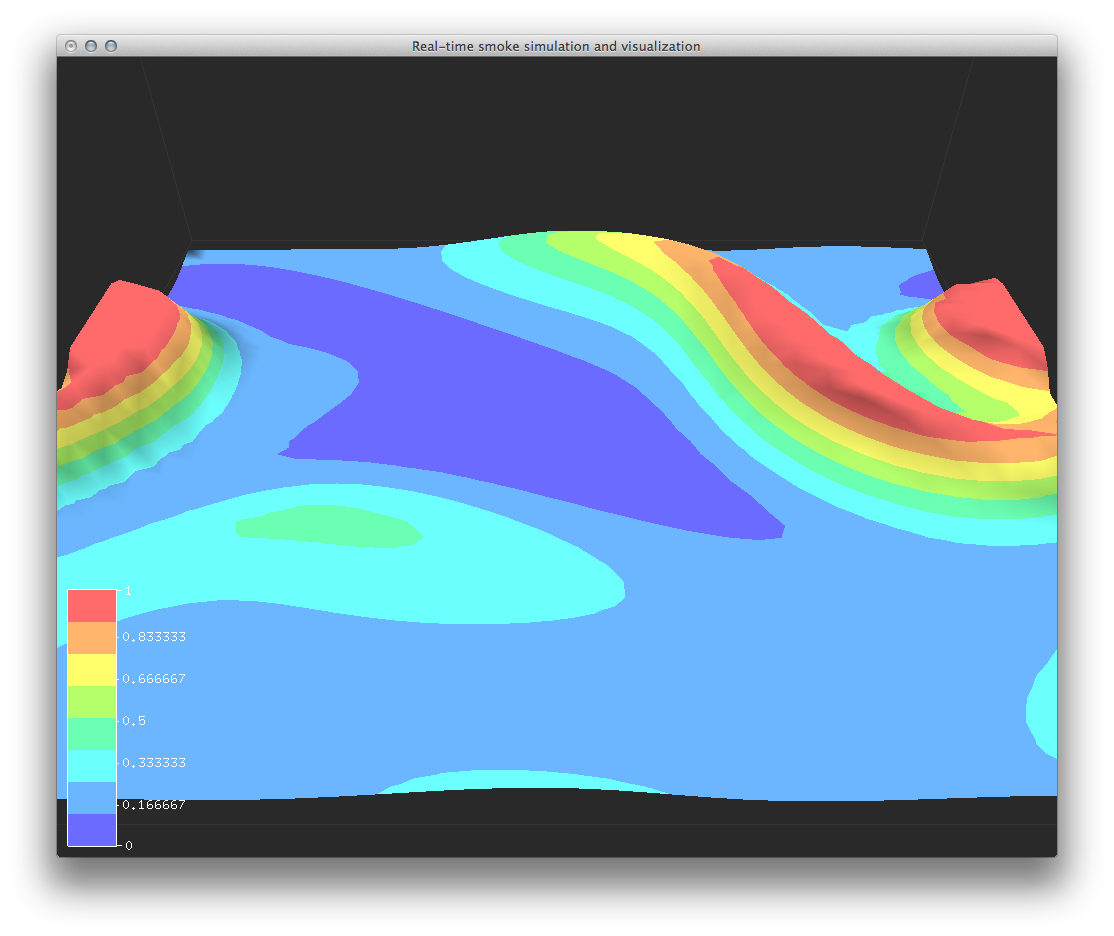
\includegraphics[height=3in]{figures/heightplot/densitydensitybanding.png}
    \caption{caption}
    \label{fig:figures_heightplot_densitydensitybanding}
\end{figure}



·        Since the height plot is a 3D structure, you have to implement appropriate shading and viewpoint selection mechanisms. In both cases, use only simple techniques, bearing in mind that this is a visualization, not a realistic rendering, assignment. For example, a Gouraud shaded plot, based on a Phong lighting model with fixed material parameters, a fixed white bi-directional light source placed above the scene and shining downwards, should be enough for lighting. For viewpoint selection, do not attempt to implement a full fledged interactive viewpoint manipulation system, as this is quite complex. Provide just a simple mechanism that, for example, lets the user turn the scene around the grid’s center, and possibly constrains the view directions to lie above the ground plane. Zooming mechanisms can also be quite limited. Think of ergonomics: the best viewpoint manipulation is done via the mouse, but it is more complex to implement. If you are unsure on how to do this, implement first a viewpoint manipulation based on classical GUI elements (e.g. sliders), after which you can go do the more challenging mouse-based manipulation

euler angles 


Finally, use the color of the plot to show a separate scalar field, via the already familiar color mapping technique. For example, the plot height can show rho, and the plot color can show | f |

